\documentclass[11pt]{article}
\usepackage[T1]{fontenc}
\usepackage{graphicx}
\usepackage{hyperref}
\usepackage[small]{titlesec}

\setlength{\oddsidemargin}{0in}
\setlength{\textwidth}{6.5in}
\setlength{\topmargin}{0in}
\setlength{\textheight}{8.5in}

\begin{document}

\title{\textbf{Detecting Type of Tennis Shots from Broadcast Video \underline{\emph{Project Update}}}}
\author{Kunal Vyas\\
    University of Massachusetts Lowell\\
  \texttt{kunal\_vyas@student.uml.edu}
  \and
  Eugene Stanley\\
  University of Massachusetts Lowell\\
  \texttt{eugene\_stanley@student.uml.edu}}
  \date{\vspace{-1ex}}
  \maketitle
  
  \section{Introduction:}
  Our project is sub-divided into three main tasks: Detecting and tracking the player, detecting and tracking the ball and then finding if the shot is a forehand or a backhand.
  \section{Progress:}
  We have so far been able to detect the player using OpenCV's HOG Descriptor method, but that computation is dropping the frame rate of the video to unsatisfactory levels. So we are tracking it using Lucas Kanade method. Once we detect the player, we set track points on him and then track it until the player is lost. And this process runs in cycles. And, we are only detecting the player in a specified region of interest. For detecting the ball and its position, we are using Hough Transform. The challenge here is to detect the moving ball, which in any frame is not a perfect circle.\\
  So far, we have been able to detect the player and we are working on tracking the player. We are able to track the ball but the detection is not always perfect. We are also going to find a way to improve these over the next few days.
  \section{Screenshots:}
  \begin{figure}[h]
  \centering
  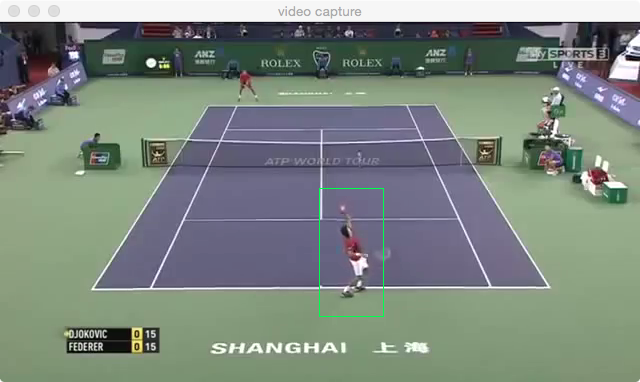
\includegraphics[width=0.4\textwidth]{1.png}
  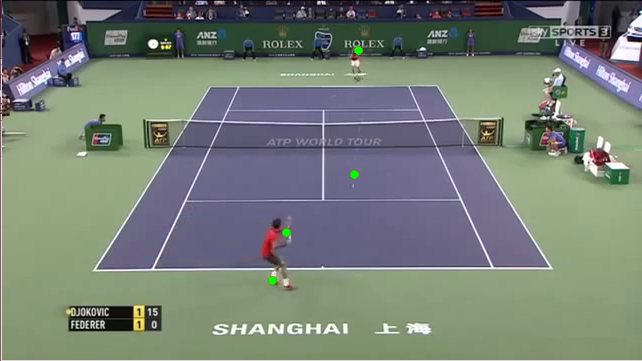
\includegraphics[width=0.4\textwidth]{3.png}
  \caption{Our program is (a) detecting the player. (b) Detecting the ball}
  \end{figure}
  \end{document}